\section{根轨迹法}

\begin{figure}[!ht]
    \centering
    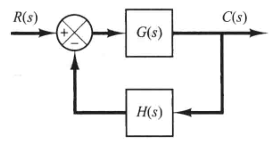
\includegraphics[width=8cm]{figures/20.png}
    \caption{闭环系统}
    \label{20}
\end{figure}

考虑如图\ref{20}所示的闭环控制系统,其传递函数为

\begin{equation*}
    \frac{C(s)}{R(s)}=\frac{G(s)}{1+G(s) H(s)}
\end{equation*}

令等式右端分母为$0$,得到特征方程:

\begin{equation*}
    1+G(s) H(s)=0
\end{equation*}

由于在$G(s)$或$H(s)$中往往存在增益$K$,可以进一步把特征方程改写为

\begin{equation*}
    1+\frac{K\left(s+z_{1}\right)\left(s+z_{2}\right) \cdots\left(s+z_{m}\right)}{\left(s+p_{1}\right)\left(s+p_{2}\right) \cdots\left(s+p_{n}\right)}=0
\end{equation*}

所谓根轨迹图,即为增益参数$K$由0编导无穷大时,闭环极点的轨迹。

典型步骤:

\begin{enumerate}
    \item 确定实轴上的根轨迹
    
    首先画出所有的开环极点与开环零点,随后根据辐角条件,确定实轴上的根轨迹。

    \item 确定渐近线
    
    \begin{align*}
        \sigma&=\frac{\sum\mbox{poles}-\sum\mbox{zeros}}{n-m}\\
        \eta_k&=\frac{(2k+1)\pi}{n-m}\quad k=0,1,2,\cdots ,n-m
    \end{align*}
\end{enumerate}